\documentclass[a4paper,oneside,12pt]{report}

\usepackage[T1]{fontenc}
\usepackage[utf8]{inputenc}
\usepackage[french]{babel}
\usepackage{lmodern}
\usepackage{microtype}
\usepackage{graphicx}
\usepackage{geometry}
\usepackage{fancyhdr}
\usepackage{hyperref}
\usepackage{caption}
\usepackage{subcaption}
\usepackage{booktabs}
\usepackage{longtable}
\usepackage{array}
\usepackage{multirow}
\usepackage{xcolor}
\usepackage{listings}
\usepackage{float}
\usepackage{enumitem}
\usepackage{csquotes}
\usepackage{makeidx}
\usepackage{pdflscape}
\usepackage{needspace}

\makeindex
\graphicspath{{assets/screenshots/}{assets/}}

\geometry{
  a4paper,
  left=2.5cm,
  right=2.5cm,
  top=2.5cm,
  bottom=2.5cm
}

\hypersetup{
  colorlinks=true,
  linkcolor=black,
  urlcolor=blue,
  citecolor=black,
  plainpages=false,
  hypertexnames=false,
  pdfpagelabels=true,
  pdftitle={Rapport de stage - IceVentes},
  pdfauthor={Walid El Kiyesse}
}

\pagestyle{fancy}
\fancyhf{}
\fancyhead[L]{\leftmark}
\fancyhead[R]{\thepage}
\fancyfoot[C]{\thepage}
\setlength{\headheight}{16pt}
\raggedbottom

\parindent 0pt
\parskip 0.5em
\setlist[itemize]{itemsep=0.2em, topsep=0.3em, parsep=0pt, partopsep=0pt}
\setlist[enumerate]{itemsep=0.2em, topsep=0.3em, parsep=0pt, partopsep=0pt}
\setlength{\floatsep}{0.45em}
\setlength{\textfloatsep}{0.6em}
\setlength{\intextsep}{0.45em}
\captionsetup{skip=0.25em}
\newcommand{\figdesc}[1]{%
  \par\noindent
  \begin{minipage}{\linewidth}
    \raggedright\small\normalfont #1
  \end{minipage}%
  \par\vspace{0.35em}%
}

\definecolor{codeblue}{RGB}{25,70,140}
\definecolor{codegray}{RGB}{110,110,110}
\definecolor{codepurple}{RGB}{110,40,120}

\lstdefinelanguage{python}{
  keywords={and,as,assert,break,class,continue,def,del,elif,else,except,False,finally,for,from,global,if,import,in,is,lambda,None,nonlocal,not,or,pass,raise,return,True,try,while,with,yield,self},
  keywordstyle=\color{codeblue}\bfseries,
  ndkeywords={models,forms,def,print},
  sensitive=true,
  comment=[l]{\#},
  commentstyle=\color{codegray}\ttfamily,
  stringstyle=\color{codepurple}\ttfamily,
  morestring=[b]',
  morestring=[b]",
  basicstyle=\ttfamily\small
}

\lstset{
  breaklines=true,
  breakatwhitespace=false,
  basicstyle=\ttfamily\small,
  frame=single,
  showstringspaces=false,
  numbers=left,
  numberstyle=\tiny\color{codegray},
  xleftmargin=2em,
  framexleftmargin=1.5em,
  inputencoding=utf8,
  extendedchars=true,
  literate=
    {à}{{\`a}}1 {â}{{\^a}}1 {ä}{{\"a}}1
    {ç}{{\c{c}}}1
    {é}{{\'e}}1 {è}{{\`e}}1 {ê}{{\^e}}1 {ë}{{\"e}}1
    {î}{{\^i}}1 {ï}{{\"i}}1
    {ô}{{\^o}}1 {ö}{{\"o}}1
    {ù}{{\`u}}1 {û}{{\^u}}1 {ü}{{\"u}}1
    {À}{{\`A}}1 {Â}{{\^A}}1 {Ä}{{\"A}}1
    {Ç}{{\c{C}}}1
    {É}{{\'E}}1 {È}{{\`E}}1 {Ê}{{\^E}}1 {Ë}{{\"E}}1
    {Î}{{\^I}}1 {Ï}{{\"I}}1
    {Ô}{{\^O}}1 {Ö}{{\"O}}1
    {Ù}{{\`U}}1 {Û}{{\^U}}1 {Ü}{{\"U}}1
    {œ}{{\oe}}1 {Œ}{{\OE}}1
}

\newcommand{\reportTitle}{Conception et réalisation d'une application web de gestion des ventes de blocs de glace}
\newcommand{\reportSubtitle}{« IceVentes » : plateforme Django pour l'Office National des Pêches}
\newcommand{\reportAuthor}{Walid El Kiyesse}
\newcommand{\reportSupervisor}{Abdelghani OUGRI}
\newcommand{\reportCompany}{Office National des Pêches (ONP)}
\newcommand{\reportSchool}{École Marocaine des Sciences de l'Ingénieur (EMSI)}
\newcommand{\reportFiliere}{Filière 3IIR --- Ingénierie Informatique et Réseaux}
\newcommand{\reportAcademicYear}{2025--2026}
\newcommand{\reportDuration}{Durée du stage : 1 mois (06 juillet -- 06 août 2026)}
\newcommand{\reportKeywords}{IceVentes, application web, Django, Python, gestion des ventes, blocs de glace, ONP, Bootstrap, HTMX, rôles, tableau de bord}
\newcommand{\reportLogoPath}{assets/EMSI_logo2.png}
\newcommand{\reportOnpLogoPath}{assets/logo_onp.png}
\renewcommand{\bibname}{Bibliographie et Nétographie}

\providecommand{\keywords}[1]{\textbf{\textit{Mots clés : }} #1}
\providecommand{\enkeywords}[1]{\textbf{\textit{Keywords: }} #1}

\begin{document}

\begin{titlepage}
\begin{center}
\large \reportSchool \\[0.25cm]
{\normalsize \reportFiliere}\\[0.7cm]

\IfFileExists{\reportLogoPath}{%
  \makebox[\textwidth]{%
    \raisebox{-0.5\height}{\includegraphics[width=0.30\textwidth]{\reportLogoPath}}%
    \hfill
    \raisebox{-0.5\height}{\includegraphics[width=0.20\textwidth]{\reportOnpLogoPath}}%
  }\\[1.2cm]
}{
  \vspace{1.2cm}
}

{\huge \textbf{Rapport de stage}}\\[0.6cm]
{\Large \reportTitle}\\[0.35cm]
{\large \reportSubtitle}\\[1.2cm]

{\Large \textbf{Réalisé par}}\\[0.3cm]
{\large \reportAuthor}\\[0.9cm]

{\large \textbf{Encadré par}}\\[0.3cm]
{\large \reportSupervisor}\\[0.9cm]

{\large \textbf{Structure d'accueil}}\\[0.3cm]
{\large \reportCompany}\\[1.6cm]

{\normalsize \reportDuration}\\[0.35cm]
Année académique \reportAcademicYear
\end{center}
\end{titlepage}

\pagenumbering{roman}
\pagestyle{plain}
\setcounter{page}{1}

\chapter*{Résumé}
\addcontentsline{toc}{chapter}{Résumé}
Ce rapport présente la conception et la réalisation d'\textbf{IceVentes}, une application web de gestion des ventes de blocs de glace développée au cours d'un stage effectué au sein de l'Office National des Pêches (ONP). Dans le secteur de la pêche, la glace en blocs est indispensable à la conservation du poisson ; sa vente aux professionnels était jusqu'alors suivie de manière manuelle, sans centralisation ni traçabilité. Le projet vise à informatiser ce processus au moyen d'une application web moderne, sécurisée et simple d'utilisation.

La solution repose sur le cadriciel Python \textbf{Django}, une interface responsive construite avec Bootstrap~5 et HTMX, une base de données relationnelle (SQLite en développement, PostgreSQL en production) et des exports bureautiques (Excel, PDF). Elle couvre l'ensemble du cycle métier : authentification et gestion des utilisateurs avec trois rôles (Administrateur, Agent, Caissier) ; paramétrage d'un référentiel d'usines à glace (code, ville, prix unitaire en DH/Kg) ; gestion des demandeurs (clients, personnes physiques ou morales, acheteurs ou vendeurs) ; saisie d'une vente avec génération automatique d'un code unique \texttt{BG\_<réf>/<année> <numéro>} et calcul automatique de la quantité ou du prix total ; enfin, un historique multicritère avec exports et un tableau de bord synthétisant l'activité (nombre de ventes, quantité vendue, chiffre d'affaires, demandeurs actifs) ainsi qu'un graphique d'évolution mensuelle.

Une attention particulière a été portée à la cohérence des données (unicité des codes, référentiel actif unique, numérotation fiable en concurrence), à la sécurité des accès (contrôle par rôle, protection contre les attaques par force brute) et à la qualité de l'expérience utilisateur. Le rapport détaille le cadre du projet, la spécification des besoins, la conception du système et sa réalisation effective, illustrée par les interfaces produites.


\vspace{0.6em}
\noindent\keywords{\reportKeywords}

\chapter*{Abstract}
\addcontentsline{toc}{chapter}{Abstract}
This report presents the design and implementation of \textbf{IceVentes}, a web application for managing ice-block sales, developed during an internship at the National Fisheries Office (Office National des Pêches, ONP). In the fishing sector, block ice is essential for preserving fish; its sale to professionals was previously tracked manually, without centralisation or traceability. The project aims to digitise this process through a modern, secure and easy-to-use web application.

The solution is built on the Python \textbf{Django} framework, a responsive interface using Bootstrap~5 and HTMX, a relational database (SQLite in development, PostgreSQL in production) and office-document exports (Excel, PDF). It covers the whole business cycle: authentication and user management with three roles (Administrator, Agent, Cashier); configuration of an ice-factory reference (code, city, unit price in MAD/Kg); management of requesters (customers, natural or legal persons, buyers or sellers); sale entry with automatic generation of a unique code \texttt{BG\_<ref>/<year> <number>} and automatic computation of quantity or total price; and finally a multi-criteria sales history with exports and a dashboard summarising activity (number of sales, quantity sold, revenue, active requesters) together with a monthly trend chart.

Particular care was taken regarding data consistency (unique codes, a single active reference, reliable numbering under concurrency), access security (role-based control, brute-force protection) and user-experience quality. The report describes the project context, the requirements specification, the system design and its actual implementation, illustrated by the produced interfaces.


\vspace{0.6em}
\noindent\enkeywords{IceVentes, web application, Django, Python, sales management, ice blocks, ONP, Bootstrap, HTMX, roles, dashboard}

\clearpage
\phantomsection
\addcontentsline{toc}{chapter}{Table des matières}
\tableofcontents
\setcounter{tocdepth}{2}
\clearpage
\phantomsection
\addcontentsline{toc}{chapter}{Liste des figures}
\listoffigures
\clearpage
\phantomsection
\addcontentsline{toc}{chapter}{Liste des tableaux}
\listoftables
\clearpage
\phantomsection
\chapter*{Liste des abréviations}
\addcontentsline{toc}{chapter}{Liste des abréviations}
\begin{longtable}{@{}p{3cm}p{11cm}@{}}
\textbf{Acronyme} & \textbf{Signification} \\
\midrule
\endfirsthead

\textbf{Acronyme} & \textbf{Signification} \\
\midrule
\endhead

API & Application Programming Interface \\
BG & Bloc de Glace \\
CIN & Carte d'Identité Nationale \\
CRUD & Create, Read, Update, Delete \\
CSS & Cascading Style Sheets \\
CSV & Comma-Separated Values \\
DH & Dirham marocain \\
HTML & HyperText Markup Language \\
HTMX & Hypertext Markup eXtensions (bibliothèque JavaScript) \\
HTTP & HyperText Transfer Protocol \\
IHM & Interface Homme-Machine \\
KPI & Key Performance Indicator (indicateur clé de performance) \\
MVC & Model-View-Controller \\
MVT & Model-View-Template \\
ONP & Office National des Pêches \\
ORM & Object-Relational Mapping \\
PDF & Portable Document Format \\
PFE & Projet de Fin d'Études \\
SGBD & Système de Gestion de Base de Données \\
SQL & Structured Query Language \\
UI & User Interface \\
UML & Unified Modeling Language \\
URL & Uniform Resource Locator \\
UX & User Experience \\
WSGI & Web Server Gateway Interface \\
\end{longtable}


\clearpage
\pagestyle{fancy}
\pagenumbering{arabic}

\chapter*{Introduction générale}
\addcontentsline{toc}{chapter}{Introduction générale}
La transformation numérique constitue aujourd'hui un levier majeur d'amélioration de la performance des organisations, y compris dans les établissements publics. En automatisant les tâches répétitives, en fiabilisant les données et en offrant une vision consolidée de l'activité, les applications de gestion permettent de gagner en efficacité, en traçabilité et en qualité de service.

C'est dans ce contexte que s'inscrit le présent stage, réalisé au sein de l'Office National des Pêches (ONP). L'ONP accompagne le développement du secteur de la pêche au Maroc et met notamment à disposition des professionnels de la glace en blocs, indispensable à la conservation du poisson depuis le débarquement jusqu'à la commercialisation. La vente de cette glace génère une activité récurrente qui, dans le cadre de ce projet, était suivie de façon essentiellement manuelle.

Cette gestion manuelle présente plusieurs limites : risque d'erreurs de saisie et de calcul, absence de numérotation fiable des tickets de vente, difficulté à retrouver l'historique des transactions, et impossibilité de disposer d'indicateurs synthétiques sur l'activité. L'objectif du stage est donc de \textbf{concevoir et réaliser une application web} qui centralise et sécurise la gestion des ventes de blocs de glace, tout en restant simple à utiliser au quotidien par les agents et caissiers.

L'application développée, baptisée \textbf{IceVentes}, couvre la gestion des utilisateurs et de leurs rôles, le paramétrage du prix de la glace, la gestion des clients, la saisie des ventes avec génération automatique d'un code unique, ainsi que la consultation de l'historique et le pilotage de l'activité à travers un tableau de bord.

Ce rapport est organisé en quatre chapitres :

\begin{itemize}
  \item le \textbf{premier chapitre} présente le cadre du projet : l'organisme d'accueil, le contexte, la problématique, les objectifs et la conduite du projet ;
  \item le \textbf{deuxième chapitre} est consacré à la spécification des besoins fonctionnels et non fonctionnels, ainsi qu'à l'identification des acteurs et des cas d'utilisation ;
  \item le \textbf{troisième chapitre} détaille la conception du système : architecture, modèle de données et diagrammes de séquence ;
  \item le \textbf{quatrième chapitre} décrit la réalisation : environnement technique, interfaces produites, fonctionnalités clés et validation.
\end{itemize}

Le rapport se termine par une conclusion générale qui dresse le bilan du travail réalisé et propose des perspectives d'évolution.


\chapter{Présentation du cadre du projet}
Ce chapitre situe le projet dans son contexte. Il présente l'organisme d'accueil, expose la problématique métier à l'origine du besoin, précise les objectifs visés et décrit la démarche adoptée pour conduire le projet.

\section{Présentation de l'organisme d'accueil}

L'\textbf{Office National des Pêches (ONP)} est un établissement public marocain placé sous la tutelle du ministère chargé de la pêche maritime. Créé en 1969, il a pour mission de contribuer au développement du secteur de la pêche, de valoriser les produits de la mer et d'organiser leur commercialisation dans des conditions de qualité, de transparence et de traçabilité \cite{onp-site}.

Parmi ses missions, l'ONP assure notamment la gestion et l'exploitation des halles aux poissons, l'organisation de la première vente du poisson, l'aménagement des points de débarquement, ainsi que la mise à disposition des professionnels d'infrastructures et de services de soutien à l'activité de pêche. La \textbf{fabrication et la distribution de glace} en font partie : la glace en blocs est un intrant essentiel de la chaîne du froid, car elle permet de préserver la fraîcheur du poisson depuis sa capture jusqu'à sa vente.

L'ONP se caractérise par une forte dimension opérationnelle et une présence sur l'ensemble du littoral marocain. Cet environnement, marqué par des exigences de fiabilité et de rigueur dans le suivi des opérations, constitue un cadre pertinent pour un projet d'informatisation d'un processus de vente.

\section{Contexte du projet}

La glace produite par les usines de l'ONP est vendue aux professionnels du secteur (mareyeurs, coopératives, sociétés de distribution, etc.). Chaque vente correspond à une quantité de glace, exprimée en kilogrammes, facturée sur la base d'un \textbf{prix unitaire} fixé par usine (en dirhams par kilogramme). Le suivi de ces ventes doit permettre d'identifier le client, de tracer chaque transaction par un numéro unique et de conserver un historique fiable.

Dans la situation initiale, ce suivi reposait largement sur des supports manuels. Cette approche, bien que fonctionnelle, atteint rapidement ses limites lorsque le volume d'opérations augmente et que le besoin de reporting se fait sentir.

\section{Problématique}

La gestion manuelle des ventes de blocs de glace soulève plusieurs difficultés :

\begin{itemize}
  \item \textbf{Fiabilité des calculs} : le calcul de la quantité à partir du prix (ou inversement) est effectué à la main, ce qui est source d'erreurs ;
  \item \textbf{Numérotation des ventes} : l'attribution d'un numéro unique et croissant à chaque ticket est difficile à garantir, surtout en cas de saisies simultanées ;
  \item \textbf{Traçabilité} : retrouver une vente passée, filtrer par période, par client ou par montant, devient fastidieux ;
  \item \textbf{Pilotage} : l'absence d'indicateurs consolidés (volume vendu, chiffre d'affaires) prive les responsables d'une vision synthétique de l'activité ;
  \item \textbf{Sécurité et rôles} : rien ne distingue formellement les personnes autorisées à créer une vente de celles qui ne doivent que la consulter.
\end{itemize}

La question centrale est donc la suivante : \emph{comment concevoir une application simple, fiable et sécurisée permettant de centraliser la gestion des ventes de blocs de glace, d'en garantir la cohérence et d'en faciliter le suivi ?}

\section{Objectifs du projet}

Pour répondre à cette problématique, le projet fixe les objectifs suivants :

\begin{itemize}
  \item centraliser la saisie et la consultation des ventes dans une application web unique ;
  \item générer automatiquement un \textbf{code de vente unique} par ticket, de la forme \texttt{BG\_<réf>/<année> <numéro>} ;
  \item automatiser le calcul entre \textbf{prix total} et \textbf{quantité} à partir du prix unitaire du référentiel ;
  \item gérer les utilisateurs selon trois \textbf{rôles} distincts (Administrateur, Agent, Caissier) ;
  \item paramétrer un référentiel d'usines à glace et gérer les clients (demandeurs) ;
  \item offrir un \textbf{historique multicritère} avec exports (Excel, PDF, impression) ;
  \item fournir un \textbf{tableau de bord} d'indicateurs et un graphique d'évolution ;
  \item garantir la cohérence des données et la sécurité des accès.
\end{itemize}

\section{Conduite et planification du projet}

Le projet a été mené selon une démarche itérative et incrémentale : après une phase de découverte de l'existant et d'analyse des besoins, les fonctionnalités ont été développées par lots successifs, chaque lot étant testé et validé avant de passer au suivant. Cette approche a permis d'obtenir rapidement une application fonctionnelle, puis de l'enrichir et de la fiabiliser au fil du temps (correctifs, audit, nouvelles fonctionnalités, documentation).

La figure~\ref{fig:gantt} présente le planning prévisionnel du stage sous la forme d'un diagramme de Gantt.

\begin{figure}[H]
  \centering
  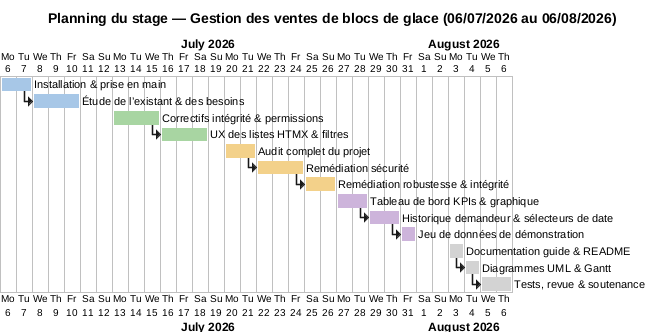
\includegraphics[width=0.98\textwidth]{gantt.png}
  \caption{Diagramme de Gantt : planification du stage}
  \label{fig:gantt}
\end{figure}
\figdesc{Le planning s'étend sur environ cinq semaines, réparties en cinq phases : découverte et analyse, correctifs et amélioration de l'expérience utilisateur, audit et remédiation, développement des fonctionnalités, puis documentation et finalisation. Chaque phase se termine par une validation avant le démarrage de la suivante.}

\section{Conclusion}

Ce chapitre a présenté le cadre du projet : l'Office National des Pêches en tant que structure d'accueil, le contexte de la vente de glace, la problématique liée à sa gestion manuelle, les objectifs à atteindre et la démarche retenue. Le chapitre suivant traduit ces objectifs en une spécification détaillée des besoins.


\chapter{Spécification des besoins}
Ce chapitre formalise les besoins auxquels l'application doit répondre. Il identifie les acteurs du système, décrit les besoins fonctionnels et non fonctionnels, puis synthétise l'ensemble à travers un diagramme de cas d'utilisation.

\section{Identification des acteurs}

L'application distingue trois profils d'utilisateurs, correspondant à des responsabilités différentes au sein du processus de vente. Le tableau~\ref{tab:acteurs} récapitule ces acteurs et leur rôle.

\begin{table}[H]
\centering
\caption{Acteurs du système et leurs responsabilités}
\label{tab:acteurs}
\begin{tabular}{@{}p{3cm}p{11cm}@{}}
\toprule
\textbf{Acteur} & \textbf{Responsabilités} \\
\midrule
Administrateur & Accès complet : gestion des utilisateurs, du référentiel et des demandeurs, création et consultation des ventes, exports et pilotage. \\
Caissier & Création et consultation des ventes, impression des tickets et exports ; pas d'accès à l'administration. \\
Agent & Consultation seule : tableau de bord et historique des ventes, sans possibilité de création ni d'export. \\
\bottomrule
\end{tabular}
\end{table}

\section{Besoins fonctionnels}

Les besoins fonctionnels sont organisés par module métier :

\begin{itemize}
  \item \textbf{Authentification et utilisateurs} : connexion sécurisée ; gestion des comptes (création, modification, activation/désactivation) ; affectation d'un rôle ; recherche et filtrage des utilisateurs.
  \item \textbf{Référentiel} : paramétrage de l'usine à glace (code, nom, ville, prix unitaire en DH/Kg, logo) ; règle d'un \textbf{seul référentiel actif} à la fois, dont le prix alimente les ventes.
  \item \textbf{Demandeurs} : gestion des clients, personnes \textbf{physiques} (nom, prénom, CIN) ou \textbf{morales} (raison sociale, représentant) ; statut \textbf{acheteur} ou \textbf{vendeur} ; activation/désactivation ; recherche multicritère.
  \item \textbf{Ventes} : saisie d'une vente par sélection d'un demandeur et saisie du prix total \textbf{ou} de la quantité, l'autre valeur étant calculée automatiquement ; génération automatique du code \texttt{BG\_<réf>/<année> <numéro>} ; impression du ticket.
  \item \textbf{Historique et pilotage} : consultation des ventes avec filtres (dates, demandeur, type, code, montant) ; exports Excel et PDF, impression ; tableau de bord avec indicateurs et graphique d'évolution.
\end{itemize}

\section{Besoins non fonctionnels}

Au-delà des fonctionnalités, l'application doit satisfaire un ensemble d'exigences de qualité :

\begin{itemize}
  \item \textbf{Sécurité} : contrôle d'accès par rôle sur chaque écran, mots de passe hachés, protection contre les tentatives répétées de connexion (verrouillage) ;
  \item \textbf{Fiabilité et cohérence} : unicité des codes de vente, numérotation correcte même en cas d'accès concurrents, unicité du référentiel actif ;
  \item \textbf{Ergonomie} : interface claire et responsive, navigation intuitive, retours visuels et messages explicites ;
  \item \textbf{Performance} : pagination des listes et réponses rapides sur les écrans de consultation ;
  \item \textbf{Portabilité} : fonctionnement sur un simple poste (base SQLite) comme sur un serveur (PostgreSQL) ;
  \item \textbf{Maintenabilité} : code structuré, séparation claire des responsabilités et documentation.
\end{itemize}

\section{Diagramme de cas d'utilisation}

La figure~\ref{fig:cas-utilisation} synthétise les interactions entre les acteurs et les fonctionnalités du système.

\begin{figure}[H]
  \centering
  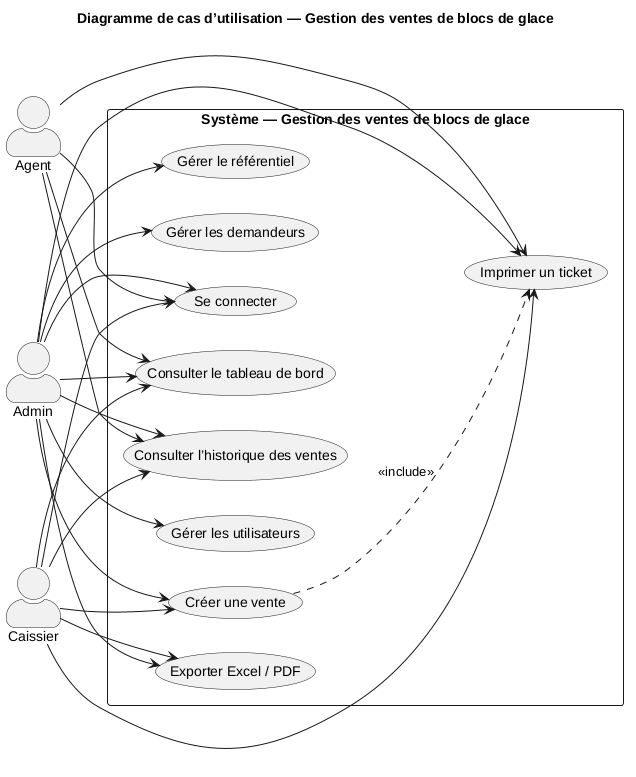
\includegraphics[width=0.72\textwidth]{cas-utilisation.png}
  \caption{Diagramme de cas d'utilisation d'IceVentes}
  \label{fig:cas-utilisation}
\end{figure}
\figdesc{Le diagramme met en évidence la séparation des droits : l'Agent est limité à la consultation (tableau de bord, historique, impression) ; le Caissier peut en plus créer des ventes et exporter ; l'Administrateur dispose de l'intégralité des fonctions, dont la gestion des utilisateurs, du référentiel et des demandeurs. La création d'une vente inclut l'impression d'un ticket.}

Le tableau~\ref{tab:droits} précise la matrice des droits par rôle.

\begin{table}[H]
\centering
\caption{Matrice des droits par rôle}
\label{tab:droits}
\begin{tabular}{@{}p{6cm}ccc@{}}
\toprule
\textbf{Fonctionnalité} & \textbf{Admin} & \textbf{Caissier} & \textbf{Agent} \\
\midrule
Se connecter & Oui & Oui & Oui \\
Tableau de bord & Oui & Oui & Oui \\
Historique des ventes & Oui & Oui & Oui \\
Créer une vente & Oui & Oui & Non \\
Exporter (Excel / PDF) & Oui & Oui & Non \\
Gérer les utilisateurs & Oui & Non & Non \\
Gérer le référentiel & Oui & Non & Non \\
Gérer les demandeurs & Oui & Non & Non \\
\bottomrule
\end{tabular}
\end{table}

\section{Conclusion}

Ce chapitre a défini les besoins fonctionnels et non fonctionnels de l'application, ainsi que les acteurs et leurs droits. Ces éléments constituent le socle de la conception présentée dans le chapitre suivant.


\chapter{Conception du système}
Ce chapitre décrit la conception de l'application : son architecture logicielle, son modèle de données et la dynamique de ses principaux scénarios, illustrée par des diagrammes de séquence. Les règles métier essentielles sont également précisées.

\section{Architecture logicielle}

L'application est bâtie sur le cadriciel \textbf{Django}, qui repose sur le patron d'architecture \textbf{MVT} (Model-View-Template), variante du modèle MVC :

\begin{itemize}
  \item le \textbf{Model} décrit les données et la logique métier ; il est projeté sur la base de données par l'ORM de Django ;
  \item la \textbf{View} traite les requêtes, applique les règles d'accès et prépare les données ;
  \item le \textbf{Template} produit les pages HTML envoyées au navigateur.
\end{itemize}

L'application suit une architecture \textbf{client-serveur} classique : le navigateur envoie des requêtes HTTP au serveur Django, qui interroge la base de données puis renvoie les pages. Côté interface, la bibliothèque \textbf{HTMX} permet d'actualiser certaines portions de page (listes filtrées, pagination, fenêtres de détail) sans recharger l'écran complet, ce qui fluidifie l'expérience tout en conservant une logique centralisée côté serveur.

Le code est organisé en modules fonctionnels (\emph{applications} Django) : \texttt{accounts} (utilisateurs et authentification), \texttt{referentiel}, \texttt{demandeurs}, \texttt{ventes} et \texttt{core} (tableau de bord et éléments partagés). Cette séparation favorise la lisibilité et la maintenabilité.

\section{Conception de la base de données}

Le modèle de données est présenté par le diagramme de classes de la figure~\ref{fig:classes}.

\begin{figure}[H]
  \centering
  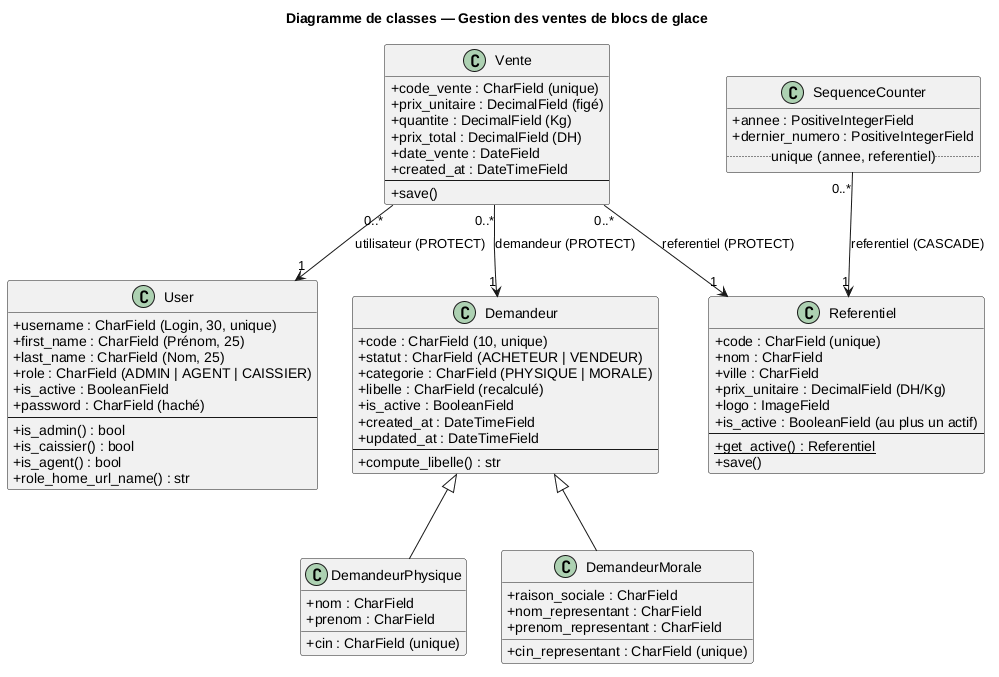
\includegraphics[width=\textwidth]{classes.png}
  \caption{Diagramme de classes d'IceVentes}
  \label{fig:classes}
\end{figure}
\figdesc{Le diagramme regroupe les entités principales : \texttt{User} (utilisateur avec rôle), \texttt{Demandeur} et ses deux spécialisations \texttt{DemandeurPhysique} et \texttt{DemandeurMorale} (héritage), \texttt{Referentiel}, \texttt{Vente} et \texttt{SequenceCounter} (compteur de numérotation). Une vente référence un demandeur, un référentiel et l'utilisateur qui l'a saisie ; ces liens sont protégés (suppression interdite) afin de préserver l'intégrité de l'historique.}

Le modèle appelle plusieurs remarques :

\begin{itemize}
  \item les demandeurs sont modélisés par \textbf{héritage} : une classe de base \texttt{Demandeur} porte les attributs communs (code, statut, catégorie), tandis que \texttt{DemandeurPhysique} et \texttt{DemandeurMorale} ajoutent leurs champs spécifiques ;
  \item le \texttt{Referentiel} porte le \textbf{prix unitaire} qui sert de référence au calcul des ventes ; une contrainte garantit qu'un \textbf{seul référentiel} est actif à la fois ;
  \item la \texttt{Vente} conserve une copie (\emph{figée}) du prix unitaire et du référentiel au moment de la vente, afin que l'historique reste exact même si le prix évolue par la suite ;
  \item le \texttt{SequenceCounter} assure une numérotation annuelle par référentiel, base de la génération du code de vente.
\end{itemize}

\section{Diagrammes de séquence}

\subsection{Authentification}

La figure~\ref{fig:seq-connexion} décrit le scénario de connexion, incluant la protection contre les tentatives répétées.

\begin{figure}[H]
  \centering
  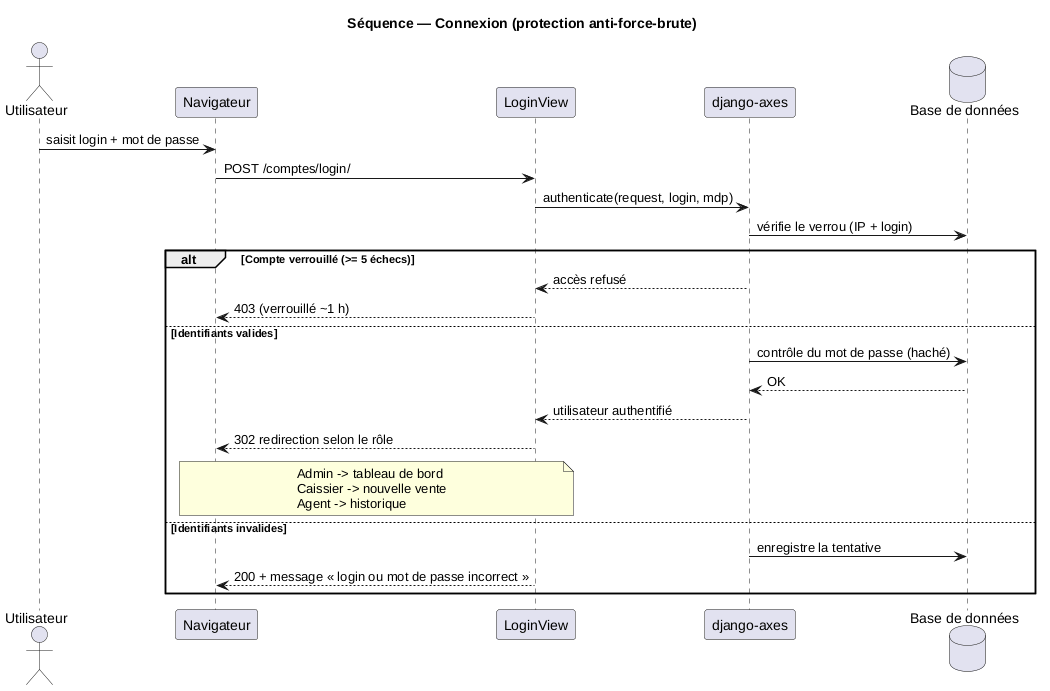
\includegraphics[width=\textwidth]{sequence-connexion.png}
  \caption{Diagramme de séquence : connexion d'un utilisateur}
  \label{fig:seq-connexion}
\end{figure}
\figdesc{L'utilisateur soumet ses identifiants ; le système vérifie d'abord qu'il n'est pas verrouillé (après plusieurs échecs), puis contrôle le mot de passe. En cas de succès, l'utilisateur est redirigé vers l'écran correspondant à son rôle ; en cas d'échec, la tentative est enregistrée et un message d'erreur est affiché.}

\subsection{Enregistrement d'une vente}

La figure~\ref{fig:seq-vente} illustre le scénario central de l'application : la saisie d'une vente et la génération de son code.

\begin{figure}[H]
  \centering
  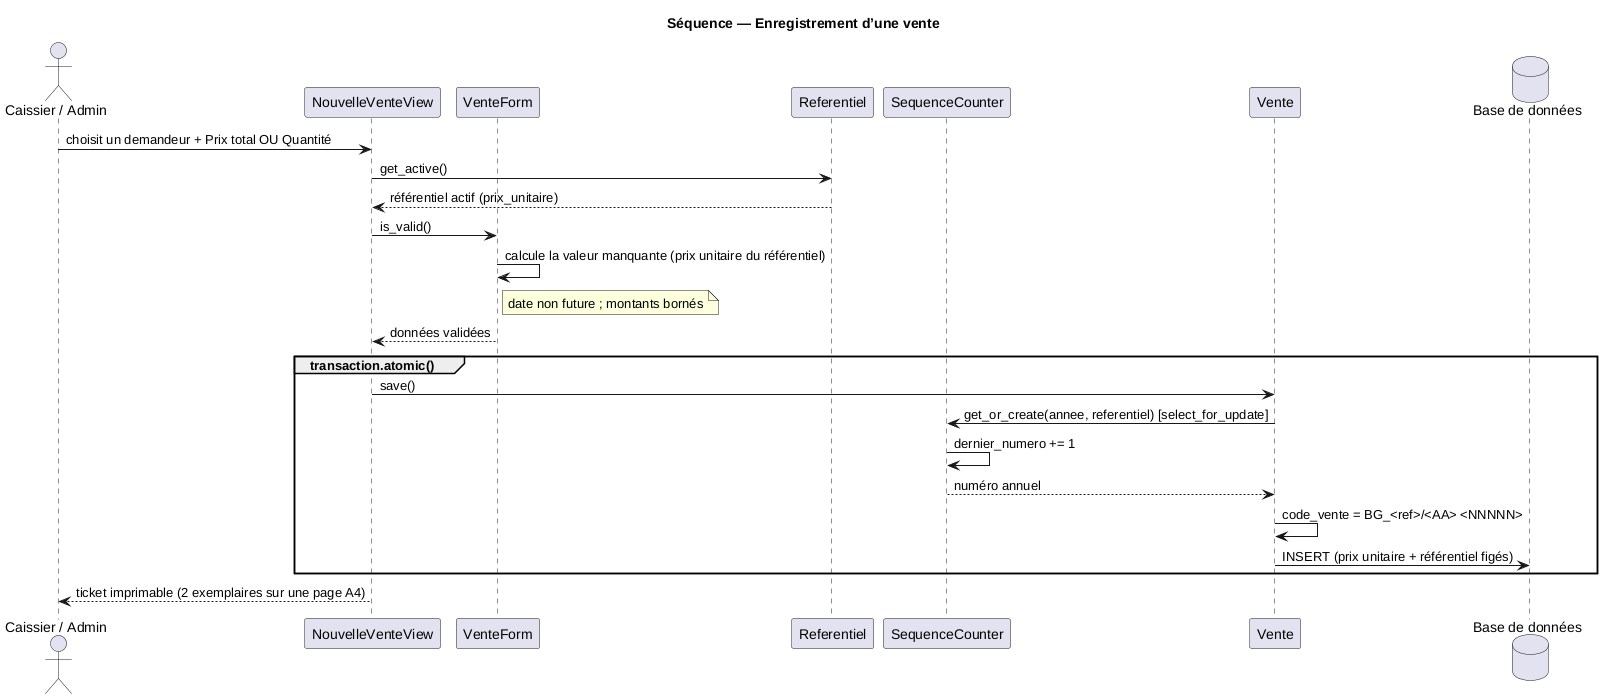
\includegraphics[width=\textwidth]{sequence-vente.png}
  \caption{Diagramme de séquence : enregistrement d'une vente}
  \label{fig:seq-vente}
\end{figure}
\figdesc{Après sélection du demandeur et saisie du prix total ou de la quantité, le système récupère le référentiel actif, calcule la valeur manquante, puis enregistre la vente dans une transaction : le compteur est incrémenté de manière verrouillée pour garantir un numéro unique, et le code \texttt{BG} définitif est attribué avant l'insertion en base. Un ticket imprimable est finalement proposé.}

\subsection{Consultation de l'historique}

La figure~\ref{fig:seq-historique} présente le filtrage de l'historique, réalisé sans rechargement complet grâce à HTMX.

\begin{figure}[H]
  \centering
  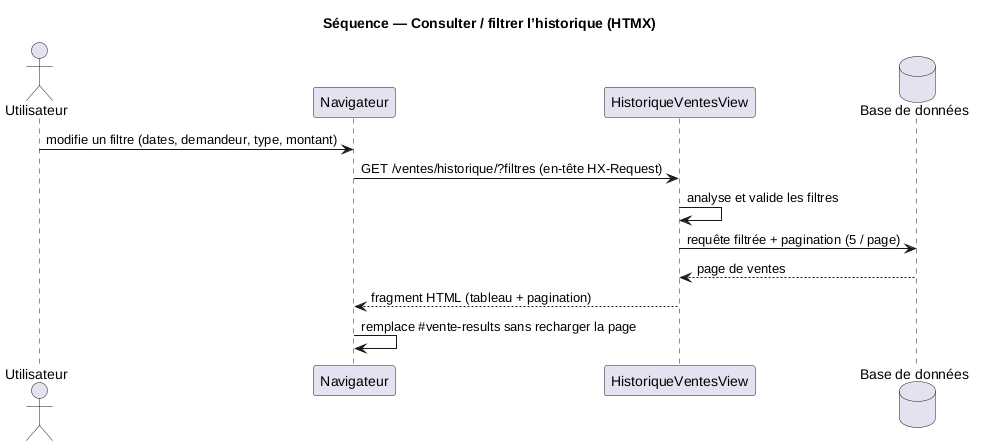
\includegraphics[width=\textwidth]{sequence-historique.png}
  \caption{Diagramme de séquence : consultation et filtrage de l'historique}
  \label{fig:seq-historique}
\end{figure}
\figdesc{Lorsque l'utilisateur modifie un filtre, une requête est envoyée au serveur, qui interroge la base avec les critères et la pagination, puis renvoie uniquement le fragment de tableau mis à jour. Le navigateur remplace la portion concernée de la page, ce qui rend l'interaction fluide.}

\section{Règles métier clés}

Trois règles structurantes garantissent la cohérence du système :

\begin{itemize}
  \item \textbf{Code de vente unique} : chaque vente reçoit un code \texttt{BG\_<réf>/<année> <numéro>}, où le numéro est croissant par année et par référentiel ; son attribution est protégée en concurrence par une transaction et un verrou ;
  \item \textbf{Référentiel actif unique} : au plus un référentiel peut être actif ; c'est son prix unitaire qui alimente toutes les nouvelles ventes ;
  \item \textbf{Cohérence des demandeurs} : le code d'un demandeur est unique, et le CIN est contrôlé de façon à éviter les doublons entre personnes physiques et morales.
\end{itemize}

\section{Conclusion}

Ce chapitre a exposé l'architecture MVT retenue, le modèle de données et les principaux scénarios dynamiques de l'application, ainsi que les règles métier garantissant sa cohérence. Le chapitre suivant présente la concrétisation de cette conception.


\chapter{Réalisation du système}
Ce chapitre présente la réalisation effective de l'application : l'environnement et les outils utilisés, les interfaces produites, une fonctionnalité clé illustrée par un extrait de code, les aspects de sécurité et enfin la validation.

\section{Environnement et outils de développement}

L'application a été développée avec un ensemble d'outils libres et éprouvés, récapitulés dans le tableau~\ref{tab:outils}.

\begin{table}[H]
\centering
\caption{Environnement technique et outils utilisés}
\label{tab:outils}
\begin{tabular}{@{}p{4.2cm}p{9.8cm}@{}}
\toprule
\textbf{Outil / Technologie} & \textbf{Rôle dans le projet} \\
\midrule
Python & Langage de programmation principal. \\
Django & Cadriciel web (ORM, routage, gabarits, administration). \\
SQLite / PostgreSQL & Base de données (développement / production). \\
HTML, CSS, Bootstrap~5 & Structure et mise en forme responsive des pages. \\
HTMX & Mises à jour partielles de page (filtres, pagination, modales). \\
Chart.js & Graphique d'évolution du chiffre d'affaires. \\
django-crispy-forms & Rendu soigné des formulaires. \\
openpyxl & Génération des exports Excel. \\
xhtml2pdf & Génération des exports PDF. \\
django-axes & Protection contre les attaques par force brute. \\
Flatpickr & Sélecteur de date au format jj/mm/aaaa. \\
UML / PlantUML & Modélisation et génération des diagrammes. \\
Git & Gestion de versions du code source. \\
\bottomrule
\end{tabular}
\end{table}

\section{Présentation des interfaces}

Cette section illustre les principaux écrans de l'application.

\subsection{Tableau de bord}

Le tableau de bord (figure~\ref{fig:dashboard}) constitue la page d'accueil ; il offre une vision synthétique de l'activité.

\begin{figure}[H]
  \centering
  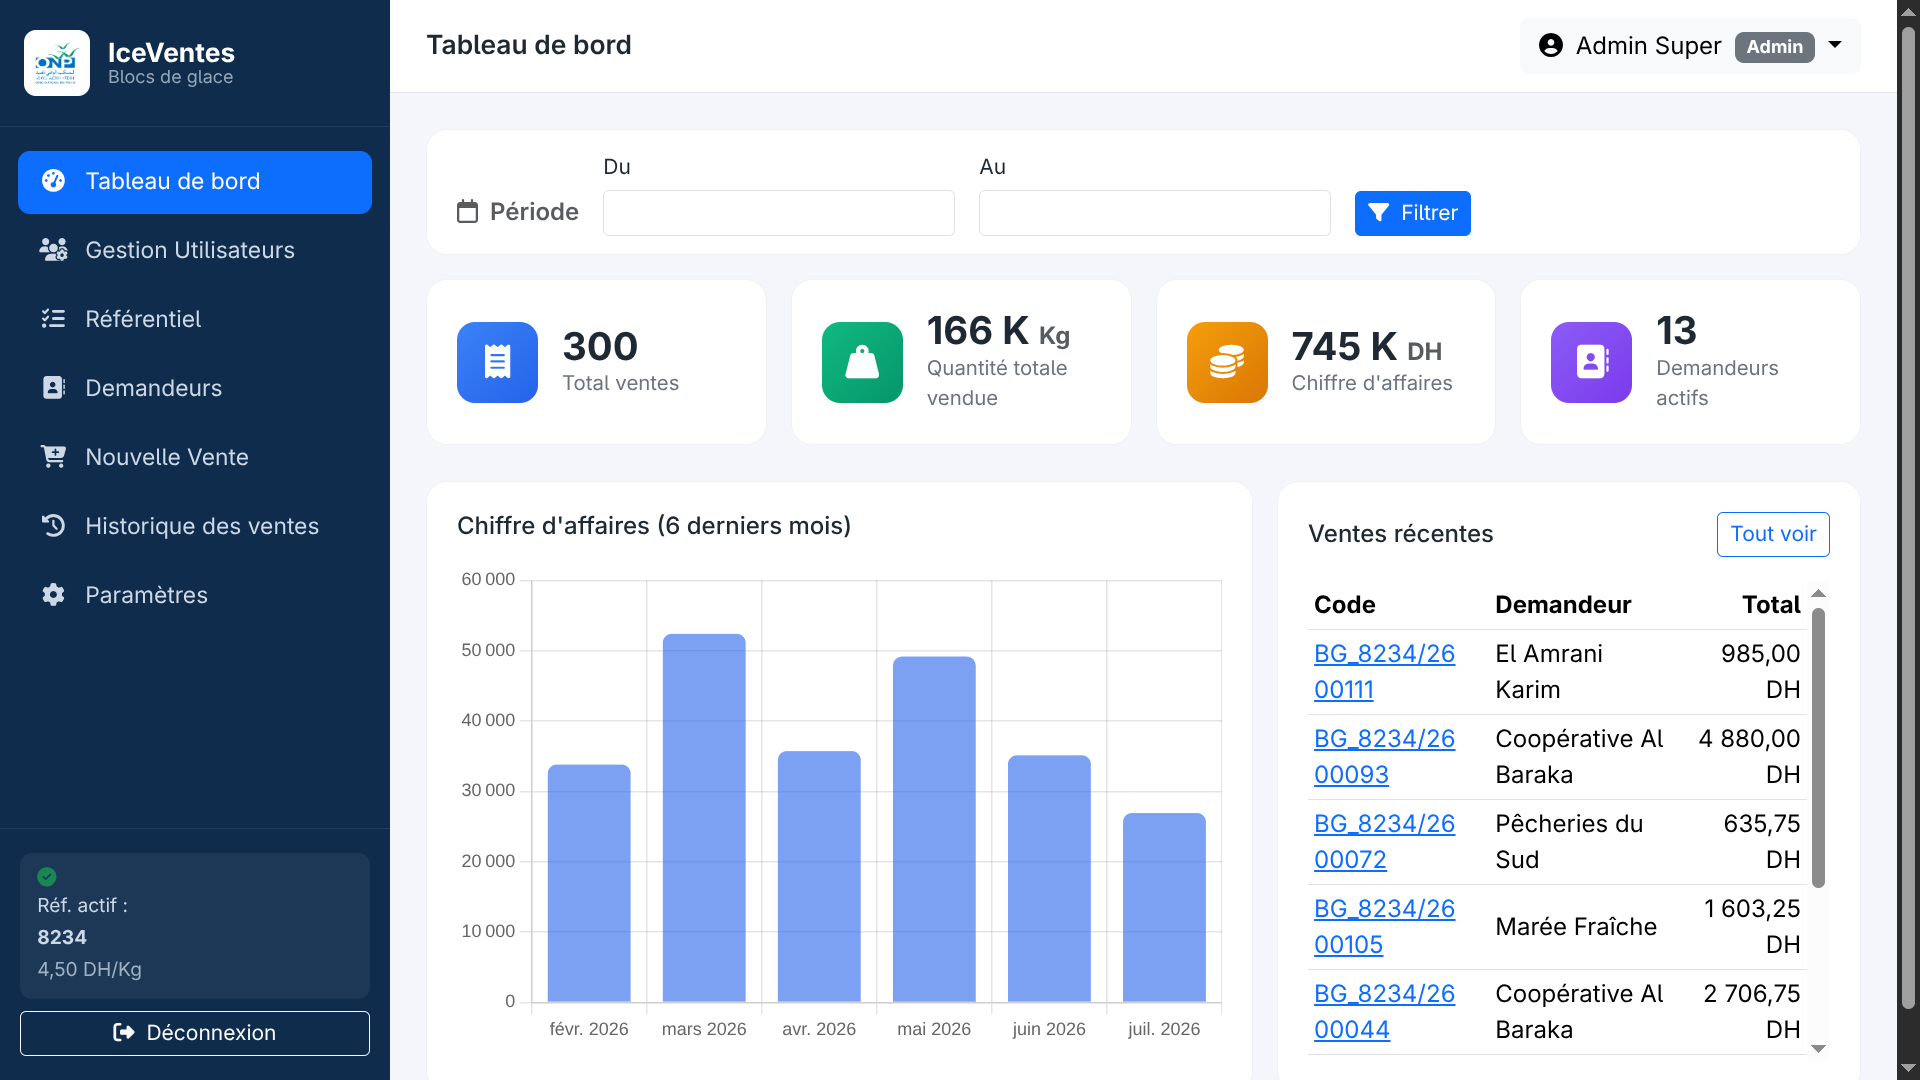
\includegraphics[width=0.95\textwidth]{tableau_de_bord.png}
  \caption{Tableau de bord : indicateurs et évolution du chiffre d'affaires}
  \label{fig:dashboard}
\end{figure}
\figdesc{Le tableau de bord affiche quatre indicateurs clés (nombre total de ventes, quantité vendue en Kg, chiffre d'affaires en DH et nombre de demandeurs actifs), présentés en notation compacte (K, M). Un graphique donne l'évolution du chiffre d'affaires sur les six derniers mois, et un panneau liste les ventes récentes. Un filtre par période permet de restreindre les statistiques à une plage de dates.}

\subsection{Gestion des utilisateurs}

L'écran de gestion des utilisateurs (figure~\ref{fig:users}) est réservé à l'administrateur.

\begin{figure}[H]
  \centering
  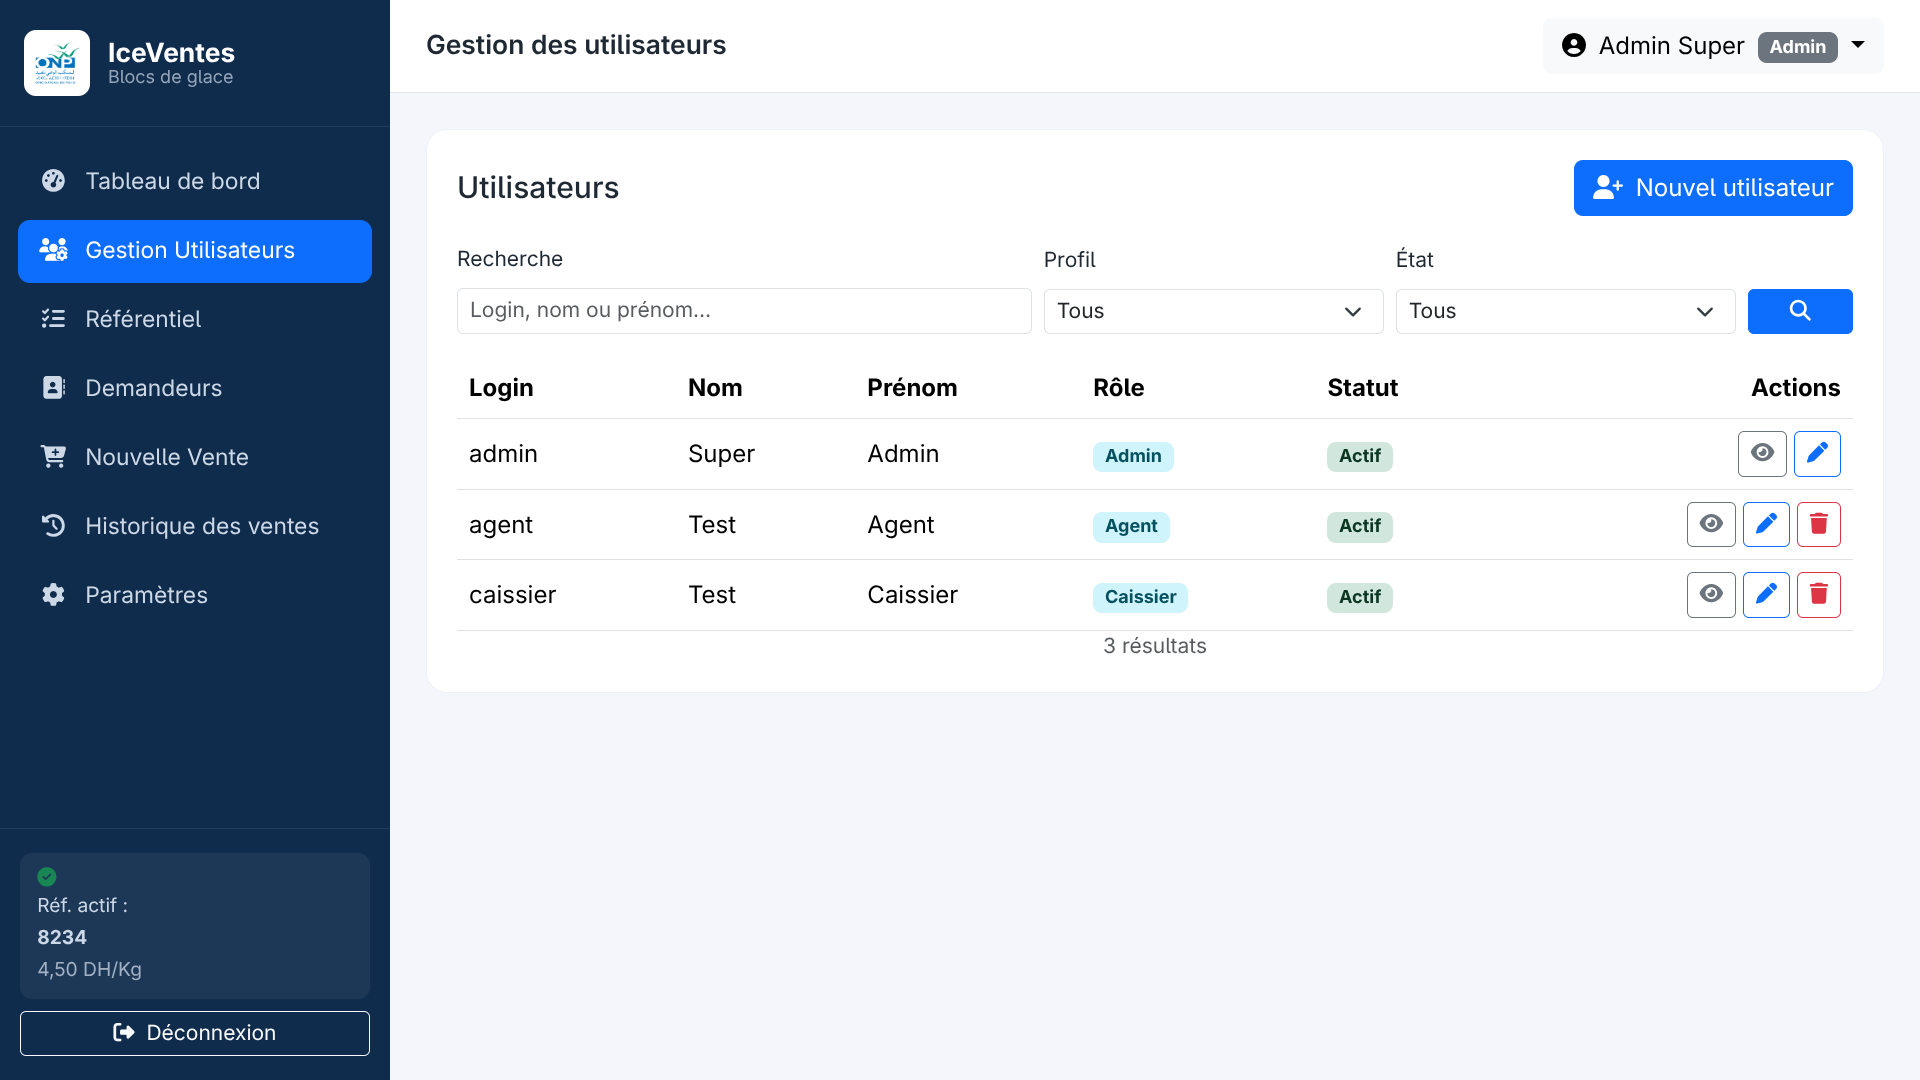
\includegraphics[width=0.95\textwidth]{gestion_utilisateurs.png}
  \caption{Gestion des utilisateurs et des rôles}
  \label{fig:users}
\end{figure}
\figdesc{La liste des utilisateurs affiche le login, le nom, le prénom, le rôle (Admin, Agent, Caissier) et le statut (actif ou désactivé). Une barre de recherche et des filtres par profil et par état facilitent la navigation. Les actions permettent de consulter, modifier et supprimer un compte, ou d'en créer un nouveau.}

\subsection{Référentiel}

Le référentiel (figure~\ref{fig:referentiel}) paramètre l'usine à glace et son prix.

\begin{figure}[H]
  \centering
  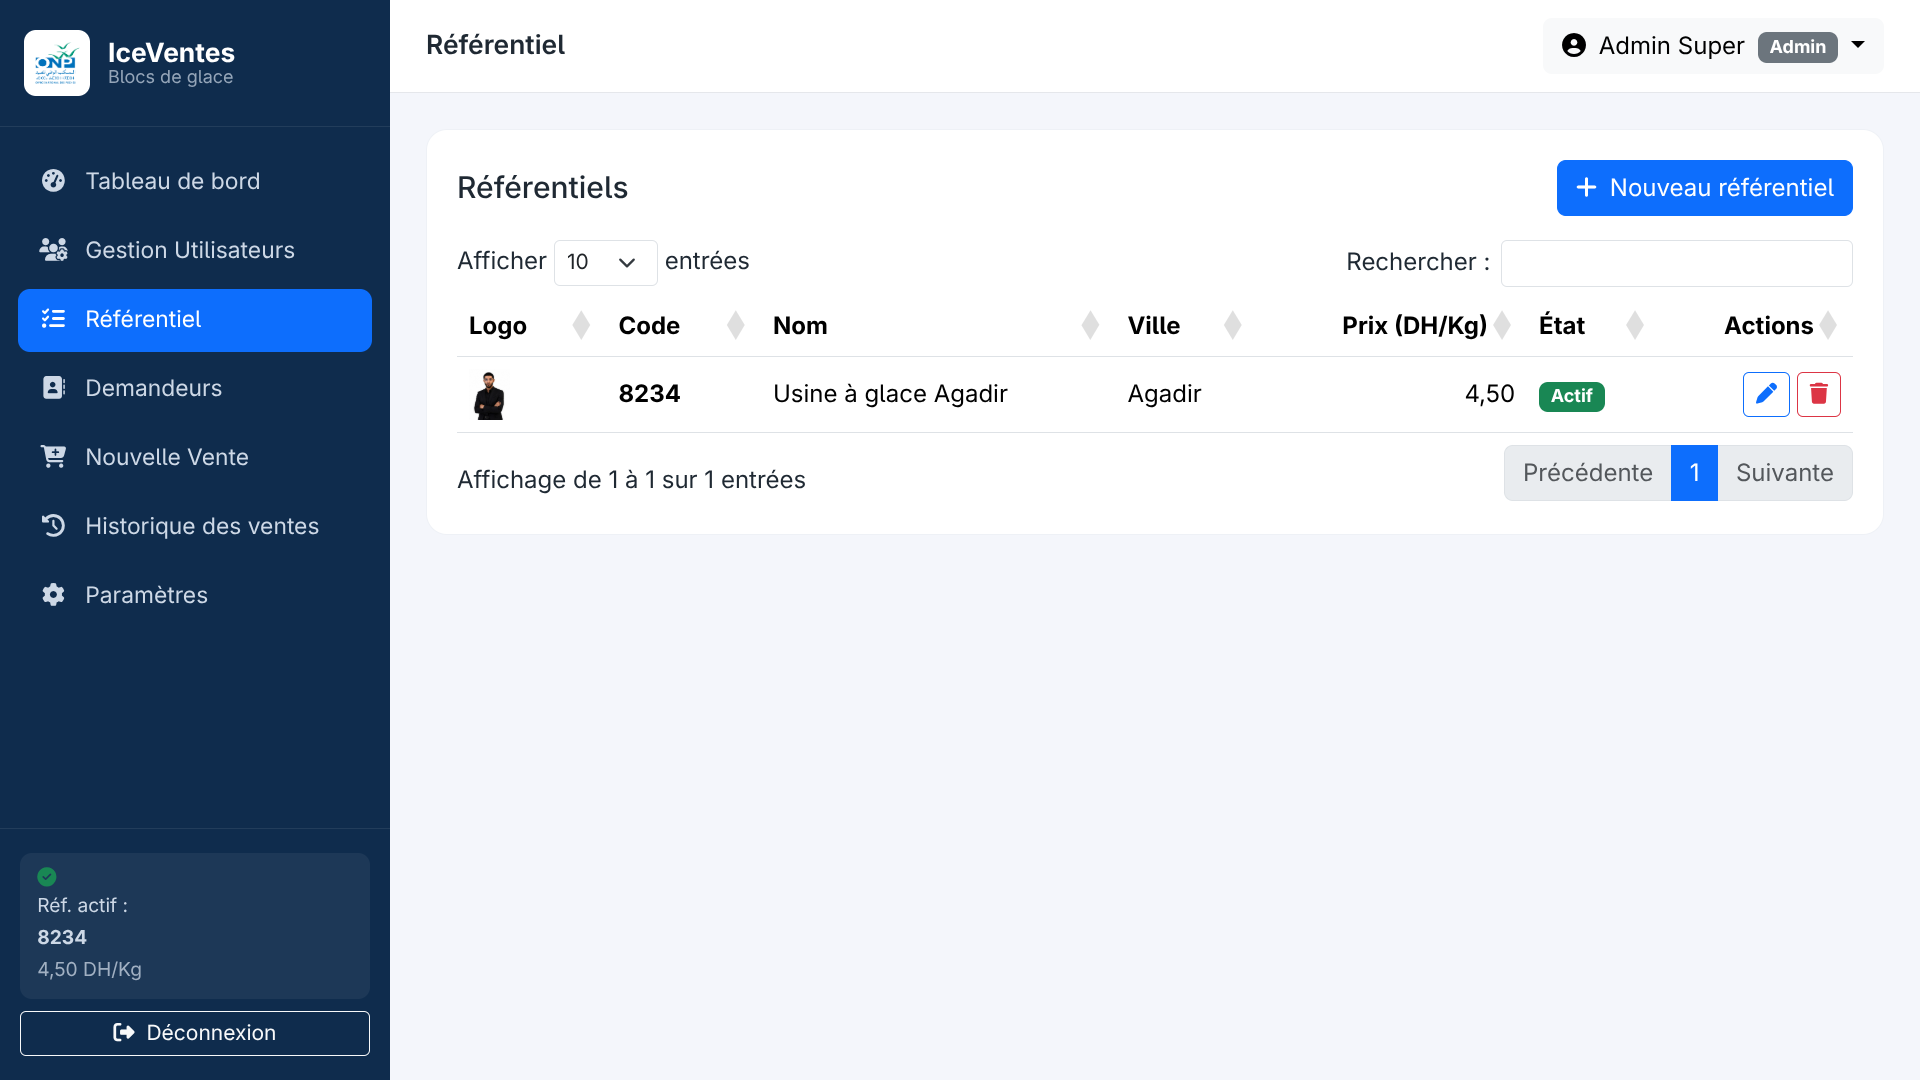
\includegraphics[width=0.95\textwidth]{referentiel.png}
  \caption{Référentiel : usine à glace et prix unitaire}
  \label{fig:referentiel}
\end{figure}
\figdesc{Le référentiel décrit l'usine à glace par un code, un nom, une ville, un logo et un prix unitaire en DH/Kg. Un seul référentiel est actif à la fois : c'est son prix (ici 4,50 DH/Kg pour l'usine d'Agadir) qui alimente automatiquement le calcul des nouvelles ventes.}

\subsection{Gestion des demandeurs}

La gestion des demandeurs (figure~\ref{fig:demandeurs}) recense les clients.

\begin{figure}[H]
  \centering
  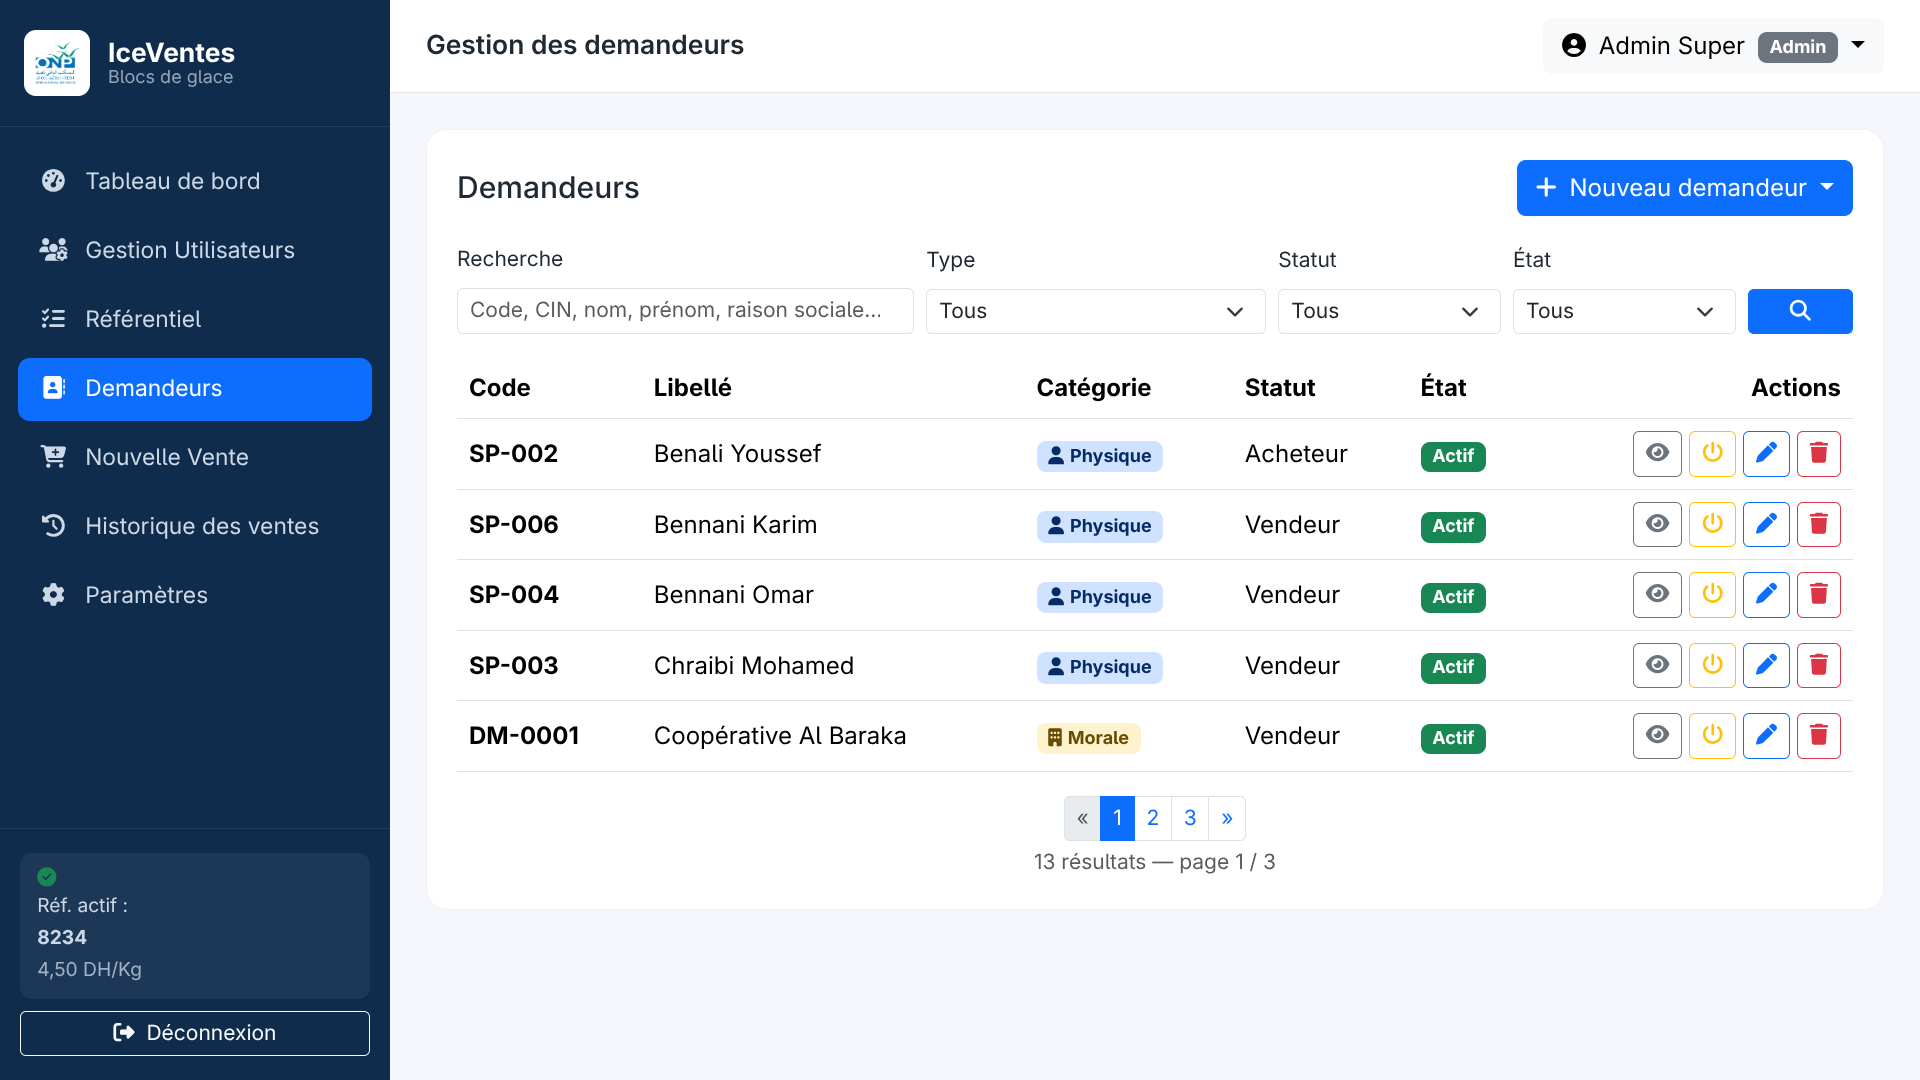
\includegraphics[width=0.95\textwidth]{demandeurs.png}
  \caption{Gestion des demandeurs (clients)}
  \label{fig:demandeurs}
\end{figure}
\figdesc{Les demandeurs peuvent être des personnes physiques ou morales, avec un statut acheteur ou vendeur. La liste, paginée, propose une recherche (code, CIN, nom, raison sociale) et des filtres par type, statut et état. Chaque demandeur peut être consulté, activé/désactivé, modifié ou supprimé.}

\subsection{Saisie d'une nouvelle vente}

L'écran de saisie (figure~\ref{fig:vente}) est au cœur de l'application.

\begin{figure}[H]
  \centering
  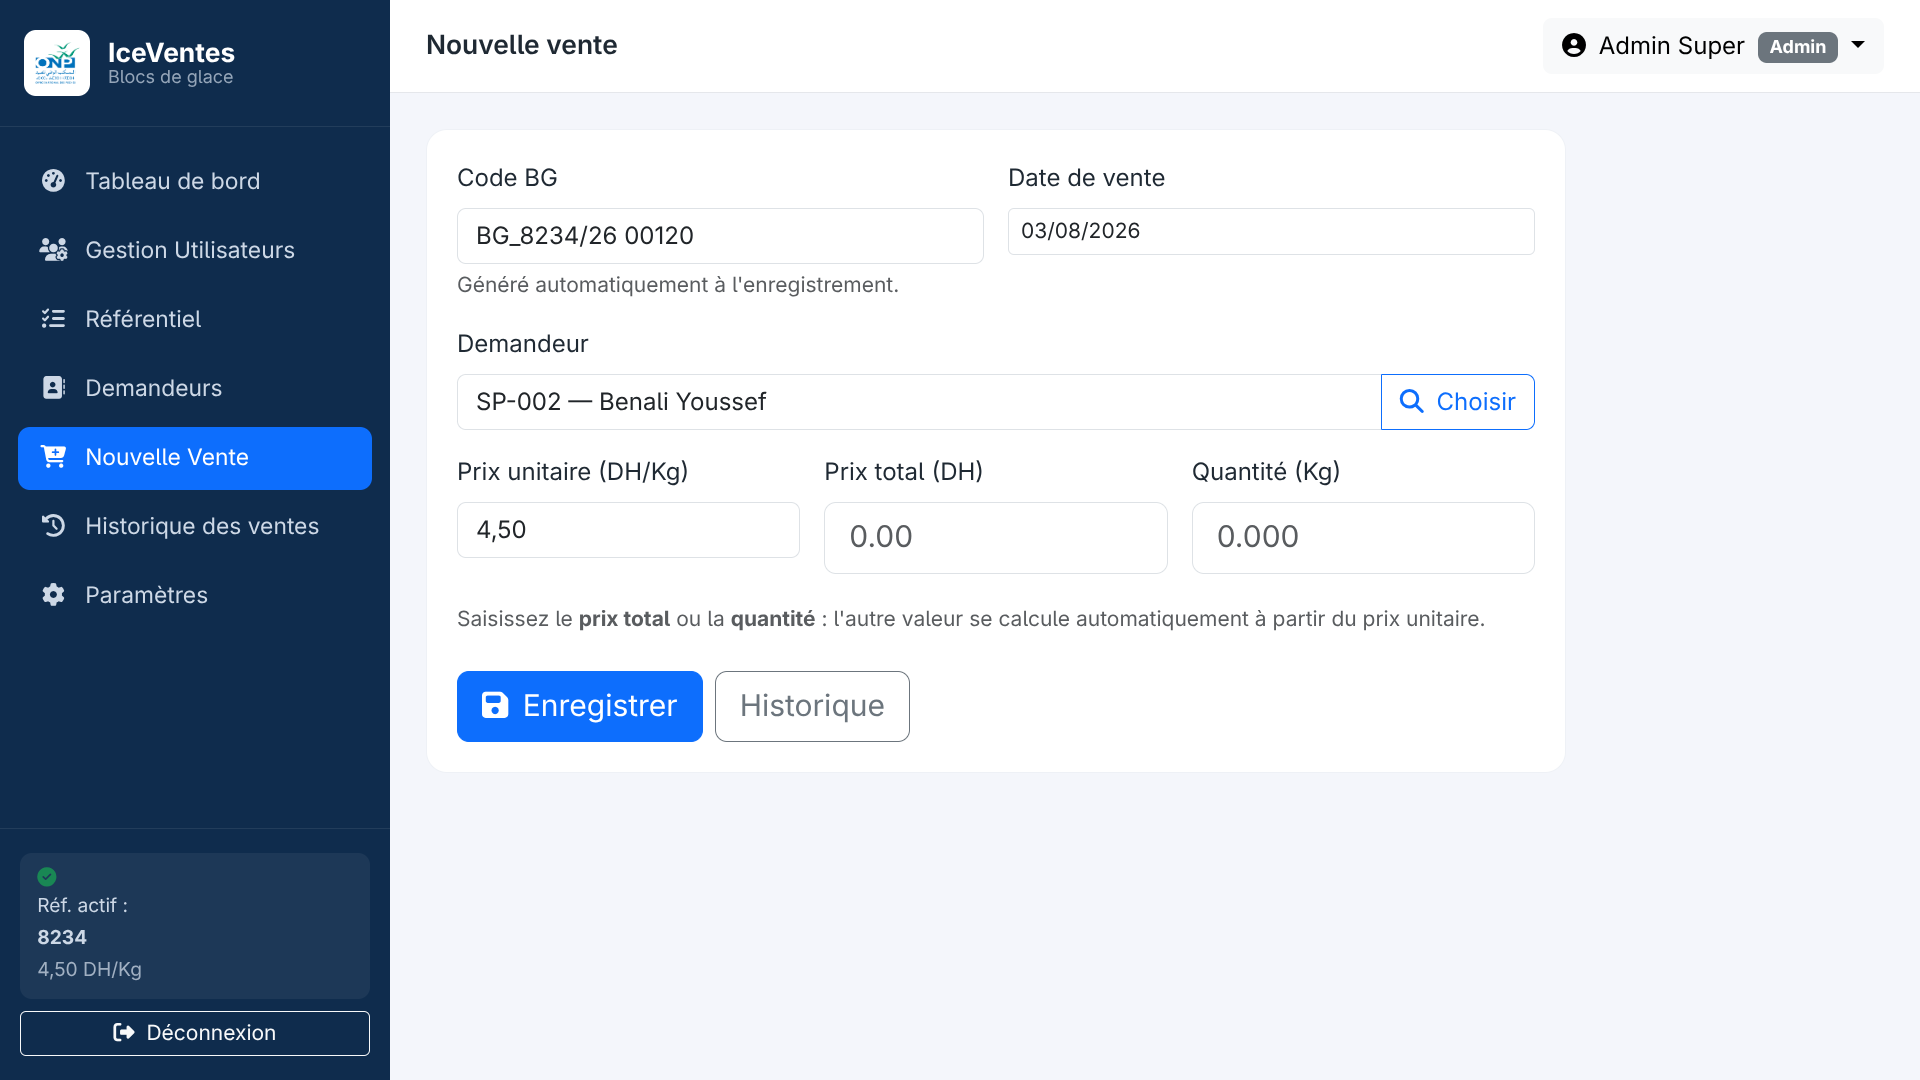
\includegraphics[width=0.95\textwidth]{nouvelle_vente.png}
  \caption{Saisie d'une nouvelle vente et génération du code BG}
  \label{fig:vente}
\end{figure}
\figdesc{Le code BG est généré automatiquement à l'enregistrement (ici \texttt{BG\_8234/26 00120}). Après avoir choisi un demandeur, l'utilisateur saisit soit le prix total, soit la quantité : l'autre valeur est calculée instantanément à partir du prix unitaire du référentiel. La date de vente et le prix unitaire sont pré-remplis.}

\subsection{Historique des ventes}

L'historique (figure~\ref{fig:historique}) permet la consultation et l'export.

\begin{figure}[H]
  \centering
  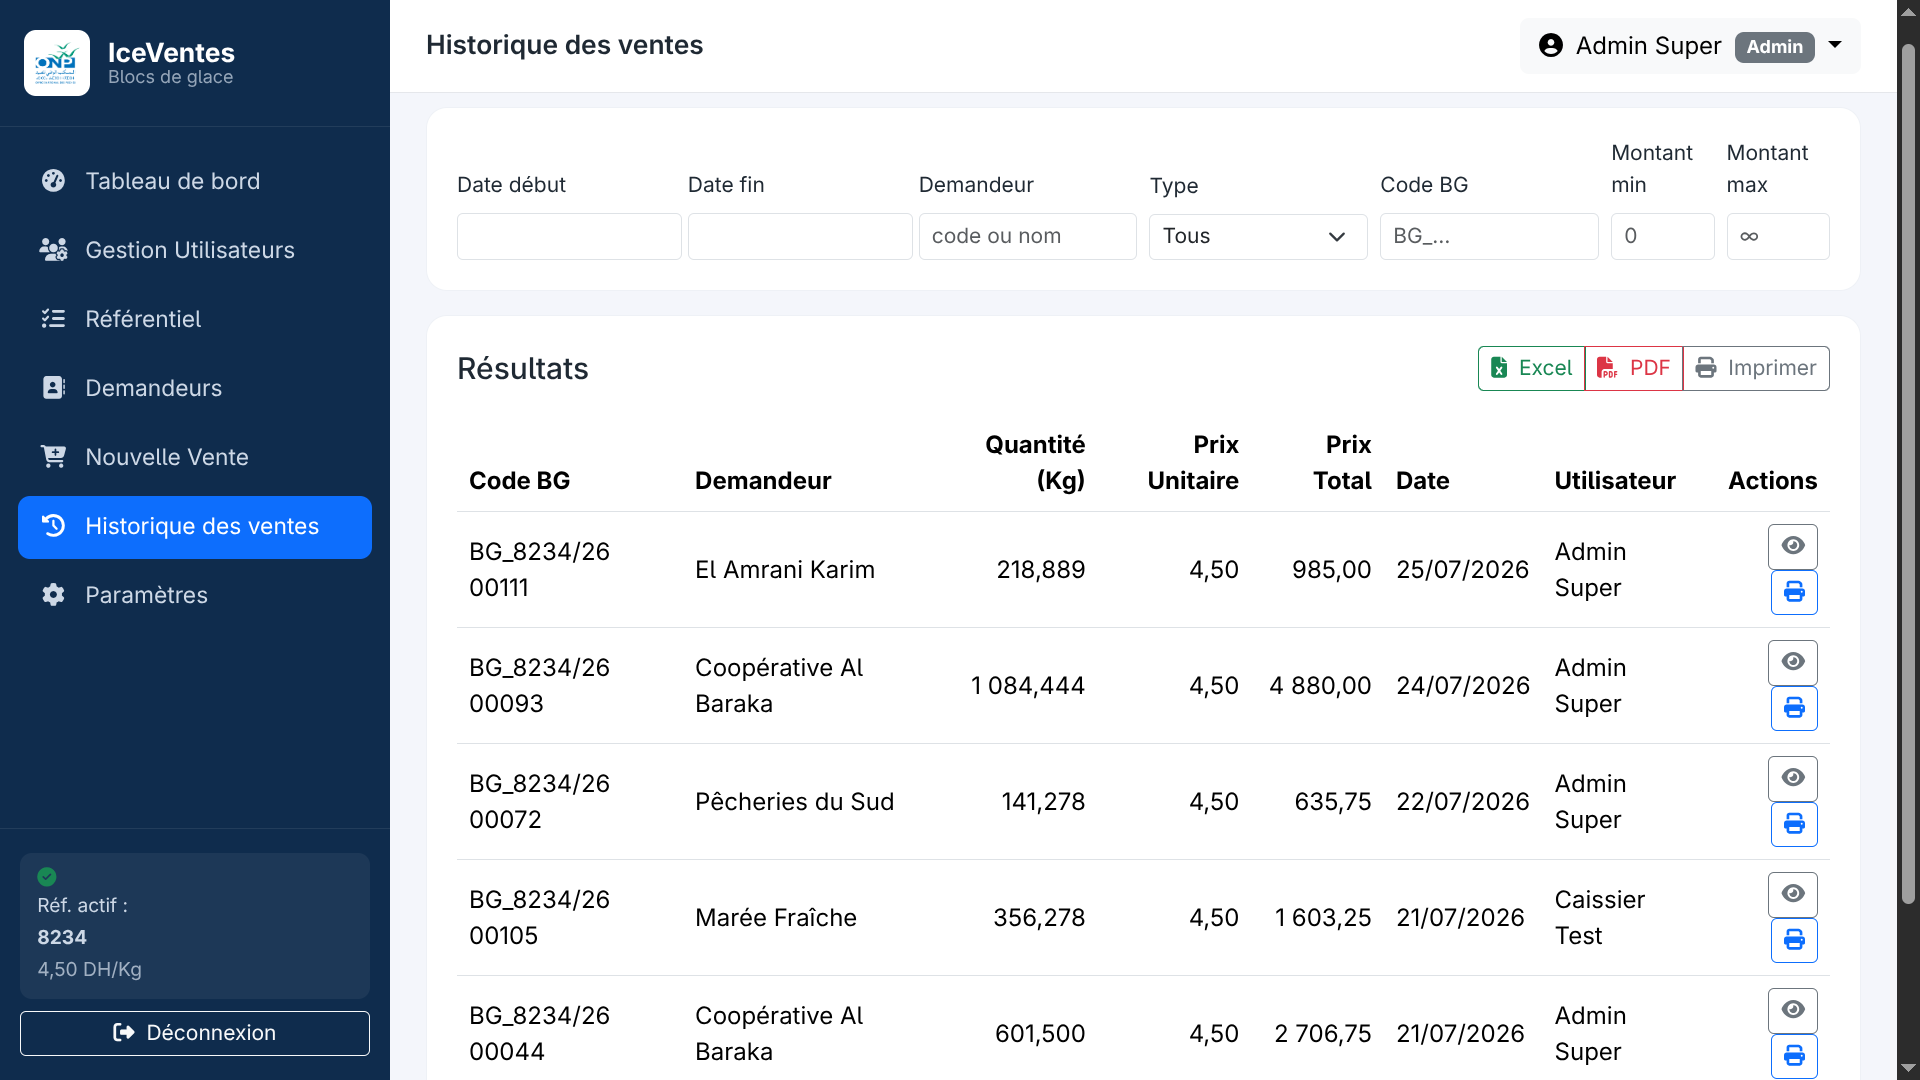
\includegraphics[width=0.95\textwidth]{historique_ventes.png}
  \caption{Historique des ventes : filtres multicritères et exports}
  \label{fig:historique}
\end{figure}
\figdesc{L'historique présente les ventes avec leur code, demandeur, quantité, prix unitaire, prix total, date et utilisateur. Une barre de filtres (dates, demandeur, type, code, montant minimum et maximum) affine les résultats sans rechargement complet. Les boutons Excel, PDF et Imprimer permettent d'exporter la sélection.}

\section{Focus sur une fonctionnalité clé : la génération du code de vente}

Le code de vente est produit par un service dédié, exécuté dans une transaction afin de garantir un numéro unique même en cas de saisies simultanées. Le compteur associé à l'année et au référentiel est verrouillé le temps de l'incrément (\texttt{select\_for\_update}). L'extrait suivant en présente le principe.

\begin{lstlisting}[language=python, caption={Génération du code de vente (principe)}, label={lst:code}]
def generer_code_vente(referentiel, date_vente):
    annee = date_vente.year
    with transaction.atomic():
        compteur, _ = SequenceCounter.objects \
            .select_for_update() \
            .get_or_create(annee=annee, referentiel=referentiel)
        compteur.dernier_numero += 1
        compteur.save(update_fields=["dernier_numero"])
        numero = compteur.dernier_numero
    aa = f"{annee % 100:02d}"
    return f"BG_{referentiel.code}/{aa} {numero:05d}"
\end{lstlisting}

Le même principe de calcul \emph{côté serveur} s'applique à la vente : la quantité et le prix total sont toujours recalculés à partir du prix unitaire du référentiel, la valeur saisie par l'utilisateur servant de point de départ. Cela évite toute incohérence et ne fait pas confiance aux valeurs éventuellement modifiées côté client.

\section{Sécurité}

Plusieurs mesures renforcent la sécurité de l'application :

\begin{itemize}
  \item \textbf{Contrôle d'accès par rôle} : chaque écran vérifie que l'utilisateur dispose des droits requis ; l'Agent, par exemple, ne peut pas accéder à la création de ventes ni aux exports ;
  \item \textbf{Protection anti-force-brute} : après plusieurs échecs de connexion, l'accès est temporairement verrouillé (django-axes) ;
  \item \textbf{Mots de passe hachés} et validation des entrées à la frontière du système ;
  \item \textbf{Intégrité des données} : unicité des codes, référentiel actif unique et numérotation fiable garantis au niveau de la base et de la logique métier.
\end{itemize}

\section{Tests et validation}

La validation a combiné des vérifications automatiques et des tests manuels des parcours par rôle. Le tableau~\ref{tab:validation} en présente une synthèse.

\begin{table}[H]
\centering
\caption{Synthèse des validations réalisées}
\label{tab:validation}
\begin{tabular}{@{}p{4.6cm}p{4.2cm}p{4.4cm}@{}}
\toprule
\textbf{Élément validé} & \textbf{Méthode} & \textbf{Résultat} \\
\midrule
Contrôle d'accès par rôle & Tests automatisés & Conforme \\
Génération du code de vente & Tests unitaires & Codes uniques et croissants \\
Calcul prix / quantité & Tests unitaires & Cohérent avec le prix unitaire \\
Référentiel actif unique & Tests + contrainte base & Un seul actif garanti \\
Filtres de l'historique & Tests fonctionnels & Résultats corrects \\
Exports Excel / PDF & Vérification fonctionnelle & Fichiers générés \\
Verrouillage anti-force-brute & Tests automatisés & Verrouillage effectif \\
\bottomrule
\end{tabular}
\end{table}

L'ensemble des tests automatisés s'exécute sans erreur, ce qui confirme la fiabilité des règles métier et des contrôles d'accès mis en place.

\section{Conclusion}

Ce chapitre a présenté la réalisation concrète d'IceVentes : son environnement technique, ses interfaces, une fonctionnalité clé, ses mécanismes de sécurité et sa validation. L'application couvre l'ensemble des objectifs fixés et fonctionne de bout en bout.


\chapter*{Conclusion générale}
\addcontentsline{toc}{chapter}{Conclusion générale}
Le stage réalisé au sein de l'Office National des Pêches avait pour objectif de concevoir et de réaliser une application web de gestion des ventes de blocs de glace, en réponse à une gestion jusqu'alors manuelle, source d'erreurs et dépourvue de traçabilité.

L'application \textbf{IceVentes} atteint cet objectif. Elle centralise l'ensemble du processus : authentification et gestion des utilisateurs selon trois rôles, paramétrage du référentiel et de son prix, gestion des demandeurs, saisie des ventes avec génération automatique d'un code unique et calcul automatisé entre prix et quantité, historique multicritère avec exports, et tableau de bord de pilotage. Une attention constante a été portée à la cohérence des données, à la sécurité des accès et à la qualité de l'expérience utilisateur.

Sur le plan personnel, ce projet a été l'occasion de mettre en pratique et d'approfondir de nombreuses compétences : la conception et la modélisation UML, le développement web avec Django, la manipulation d'une base de données relationnelle, la construction d'interfaces responsives et interactives, ainsi que la prise en compte des exigences de sécurité et de fiabilité propres à une application de gestion. Le travail dans un cadre professionnel a également renforcé la rigueur, l'autonomie et la capacité à structurer un projet de bout en bout.

Plusieurs \textbf{perspectives} d'évolution peuvent être envisagées :

\begin{itemize}
  \item la mise en production sur une base PostgreSQL et un serveur dédié ;
  \item la prise en charge de plusieurs usines à glace actives simultanément ;
  \item l'enrichissement du reporting (statistiques avancées, comparaisons, export planifié) ;
  \item l'ajout d'une gestion fine des paiements et des encaissements ;
  \item le développement d'une version mobile pour la saisie sur le terrain.
\end{itemize}

En définitive, IceVentes constitue une base solide, fonctionnelle et extensible, qui répond aux besoins exprimés tout en ouvrant la voie à des améliorations futures.


\clearpage
\addcontentsline{toc}{chapter}{Bibliographie et Nétographie}
\begin{thebibliography}{9}

\bibitem{onp-site}
Office National des Pêches (ONP).
\textit{Site officiel de l'Office National des Pêches}.
\url{http://www.onp.co.ma/}. Consulté en août 2026.

\bibitem{django}
Django Software Foundation.
\textit{Django Documentation}.
\url{https://docs.djangoproject.com/}. Consulté en août 2026.

\bibitem{python}
Python Software Foundation.
\textit{Python Language Documentation}.
\url{https://docs.python.org/3/}. Consulté en août 2026.

\bibitem{bootstrap}
Bootstrap.
\textit{Bootstrap 5 Documentation}.
\url{https://getbootstrap.com/docs/5.3/}. Consulté en août 2026.

\bibitem{htmx}
HTMX.
\textit{HTMX Documentation}.
\url{https://htmx.org/docs/}. Consulté en août 2026.

\bibitem{chartjs}
Chart.js.
\textit{Chart.js Documentation}.
\url{https://www.chartjs.org/docs/}. Consulté en août 2026.

\bibitem{axes}
django-axes.
\textit{django-axes Documentation}.
\url{https://django-axes.readthedocs.io/}. Consulté en août 2026.

\bibitem{openpyxl}
openpyxl.
\textit{openpyxl Documentation}.
\url{https://openpyxl.readthedocs.io/}. Consulté en août 2026.

\bibitem{postgresql}
PostgreSQL Global Development Group.
\textit{PostgreSQL Documentation}.
\url{https://www.postgresql.org/docs/}. Consulté en août 2026.

\bibitem{plantuml}
PlantUML.
\textit{PlantUML Language Reference Guide}.
\url{https://plantuml.com/}. Consulté en août 2026.

\end{thebibliography}


\end{document}
